% Auto-generated by the analysis pipeline — do not edit
% y > 0: Overreacts  |  y < 0: Underreacts
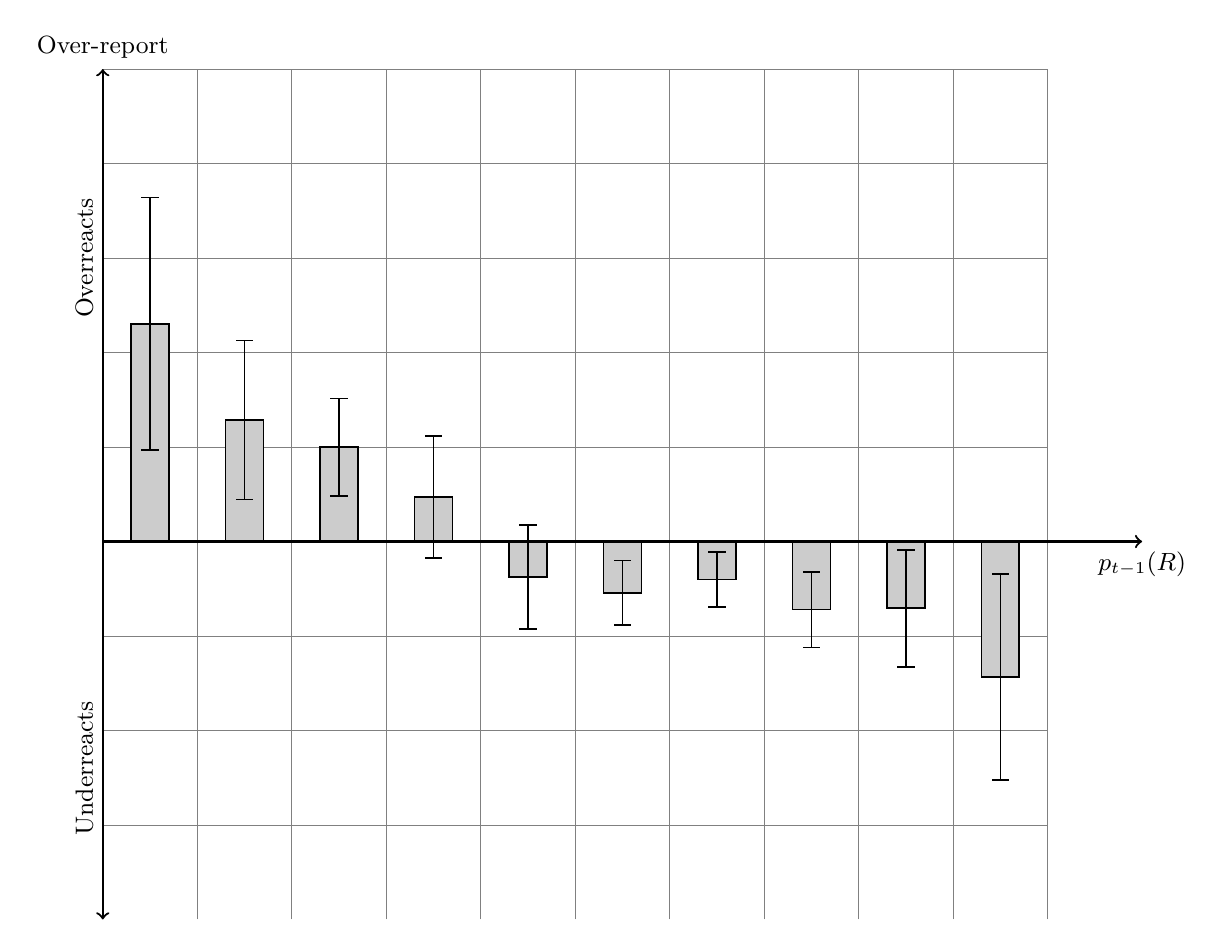
\begin{tikzpicture}[scale=12]
\draw[help lines,step=0.1] (0,-0.4) grid (1,0.5);
\filldraw[opaque,white!80!black] (0.03,0) rectangle (0.07,0.2304);
\draw[line width=0.6] (0.03,0) rectangle (0.07,0.2304);
\draw[line width=0.6,|-|] (0.05,0.0959) -- (0.05,0.3650);
\filldraw[opaque,white!80!black] (0.13,0) rectangle (0.17,0.1286);
\draw[line width=0.6] (0.13,0) rectangle (0.17,0.1286);
\draw[line width=0.6,|-|] (0.15,0.0435) -- (0.15,0.2138);
\filldraw[opaque,white!80!black] (0.23,0) rectangle (0.27,0.0997);
\draw[line width=0.6] (0.23,0) rectangle (0.27,0.0997);
\draw[line width=0.6,|-|] (0.25,0.0472) -- (0.25,0.1522);
\filldraw[opaque,white!80!black] (0.33,0) rectangle (0.37,0.0472);
\draw[line width=0.6] (0.33,0) rectangle (0.37,0.0472);
\draw[line width=0.6,|-|] (0.35,-0.0183) -- (0.35,0.1127);
\filldraw[opaque,white!80!black] (0.43,0) rectangle (0.47,-0.0377);
\draw[line width=0.6] (0.43,0) rectangle (0.47,-0.0377);
\draw[line width=0.6,|-|] (0.45,-0.0936) -- (0.45,0.0182);
\filldraw[opaque,white!80!black] (0.53,0) rectangle (0.57,-0.0543);
\draw[line width=0.6] (0.53,0) rectangle (0.57,-0.0543);
\draw[line width=0.6,|-|] (0.55,-0.0894) -- (0.55,-0.0191);
\filldraw[opaque,white!80!black] (0.63,0) rectangle (0.67,-0.0401);
\draw[line width=0.6] (0.63,0) rectangle (0.67,-0.0401);
\draw[line width=0.6,|-|] (0.65,-0.0703) -- (0.65,-0.0099);
\filldraw[opaque,white!80!black] (0.73,0) rectangle (0.77,-0.0720);
\draw[line width=0.6] (0.73,0) rectangle (0.77,-0.0720);
\draw[line width=0.6,|-|] (0.75,-0.1129) -- (0.75,-0.0312);
\filldraw[opaque,white!80!black] (0.83,0) rectangle (0.87,-0.0707);
\draw[line width=0.6] (0.83,0) rectangle (0.87,-0.0707);
\draw[line width=0.6,|-|] (0.85,-0.1335) -- (0.85,-0.0079);
\filldraw[opaque,white!80!black] (0.93,0) rectangle (0.97,-0.1436);
\draw[line width=0.6] (0.93,0) rectangle (0.97,-0.1436);
\draw[line width=0.6,|-|] (0.95,-0.2534) -- (0.95,-0.0338);
\draw[line width=0.8,->]  (0,0) -- (1.1,0) node[below] {\small{$p_{t-1}(R)$}};
\draw[line width=0.8,<->] (0,-0.4) -- (0,0.5) node[above] {\small{Over-report}};
\draw (0,0.30) node[above,rotate=90] {\small{Overreacts}};
\draw (0,-0.24) node[above,rotate=90] {\small{Underreacts}};
% ADD THEORY CURVE BELOW
\end{tikzpicture}
